\documentclass[letterpaper,12pt]{report}
\usepackage{fullpage}
\usepackage{amsmath, amsthm, amssymb}
\usepackage{graphicx}
\usepackage{verbatim}
\usepackage{fancyhdr}
\usepackage[colorlinks=true,linkcolor=blue]{hyperref}
\usepackage[all]{xy}
\usepackage{tikz}
\usepackage{caption}

\newtheorem{definition}{Definition}[chapter]
\newtheorem{theorem}{Theorem}[chapter]
\theoremstyle{plain}
\newtheorem*{thmHop}{The hopping immunity theorem}
\theoremstyle{definition}
\newtheorem*{example}{Example}

\graphicspath{{Images/}}
 
\renewcommand\topfraction{.9}
\renewcommand\textfraction{.05}
\makeatletter
\begin{comment}
\renewcommand\chapter{\if@openright\cleardoublepage\else\clearpage\fi
                    \thispagestyle{fancy}%
                    \global\@topnum\z@
                    \@afterindentfalse
                    \secdef\@chapter\@schapter}
                    \end{comment}
\makeatother

\title{\textbf{The Phase Space of Block Withholding Mining Strategies}}

\author{Assaf Shomer\\
}

\date{\today}

\begin{document}

\maketitle
%\pagestyle{fancy}
\begin{abstract}
We calculate the probability of success of block-withholding mining strategies in bitcoin-like networks.
These strategies involve building a secret branch of the block-tree and publishing it opportunistically, aiming to replace the top of the main-branch and rip the reward associated with the secretly mined blocks. We identify two types of block-withholding strategies and chart the parameter space where those are more beneficial than the standard mining strategy described in Nakamoto's paper.
Our analysis suggests a generalization of the notion of the relative hashing power as a measure for a miner's influence on the network. Block withholding attacks start becoming beneficial only when this measure of influence exceeds a certain threshold.


\end{abstract}
\pagenumbering{roman}
\tableofcontents
\chapter{Introduction}\label{chap:intro}
\pagenumbering{arabic}
\section{Bitcoin and mining}
Bitcoin is the world's first decentralized digital currency (\cite{Bitcoin}). blah blah

Motivated by the work done in \cite{Selfish} we are interested in finding out if and when the block-withholding strategy gives the miner a higher probability of success in mining blocks, compared to the standard strategy outlined in the bitcoin protocol. 

\chapter{Three mining strategies}\label{chap:strategies}

\section{The Standard Mining Strategy}
The standard mining strategy follow the bitcoin protocol described in \cite{Bitcoin}. Such miners publish each block as soon as it is discovered and switch their mining efforts to the head of the blockchain\footnote{In practice different miners may be aware of different branches of the block-tree at a given moment. Such differences are resolved with very high probability once a new block is found because the protocol names the branch with the maximal difficulty to be the blockchain.} as soon as they become aware of a new valid block.

\begin{equation}\label{theblockchain}\nonumber
\dots\rightarrow\mathit{B}_L\rightarrow\mathit{B}_{L+1}\rightarrow\mathit{B}_{L+2}\rightarrow\dots
\end{equation}

\section{Block Withholding Strategies}
Miners following this type of mining strategies do not share newly found blocks and instead work on extending a $\bf{secret}$ branch of the block-tree. The miners publish their secret branch when it is most beneficial to them. 

\begin{eqnarray}\label{fig:blockwithholdingchain}
 \dots \rightarrow \mathit{B}_L\rightarrow &\mathit{B}_{L+1}\rightarrow\mathit{B}_{L+2}
\rightarrow\dots\rightarrow\mathit{B}_{L+n} \qquad\qquad \mathrm{Main}\\\nonumber
\searrow & \\\nonumber
\qquad \qquad \qquad & \widetilde{\mathit{B}}_{L+1}\rightarrow\widetilde{\mathit{B}}_{L+2}
\longrightarrow \quad \dots \longrightarrow\widetilde{\mathit{B}}_{L+m}\qquad \mathrm{Secret}
\end{eqnarray}

\subsection{Type I (try to win)}
The miners mine their secret branch until it is \textit{longer than the main branch}. At this time they can publish it and uproot the last $n$ blocks mined by the Standard miners in favour of their $m>n$ secretly mined ones.

\subsection{Type 0 (reach a tie and get some help)}
The miners mine their secret branch until it is of the  \textit{same length as the main branch}. At this time they publish it. Now the network is bifurcated. The type 0 miners joined by some of the standard miners will mine on top of the newly published Type 0 branch. The rest of the standard miners continue working on the standard branch. If the former manage to find a new block first then the Type 0 strategy was successful. 

\section{Our Goal}\label{subsec:goal}

Our goal is to analyse which mining strategy is the most beneficial as a function of the miner's relative hashing power and the portion of standard miners that join them, in case of a Type 0 strategy.
To that effect we calculate the probability that a block-withholding miner succeeds in replacing a block (and possibly some number of confirmation blocks on top of it) by publishing a secretly mined branch of the block-tree.

\chapter{Calculation}\label{chap:calc}

\section{Setup}\label{calcsetup}
Let us denote by $\mathcal{H}$ the total hashing power of the network and divide it abstractly into a \emph{Standard} part which holds a portion $p\mathcal{H}$ of the total hashing power (where $p \in [0,1]$) and a \emph{Block Withholding} part, which holds the rest $q\mathcal{H}=(1-p)\mathcal{H}$. 

We start our analysis at a given point in time where the blockchain is of length $L$ and denote the last block mined as $\mathit{B}_L$. As time marches on the Standard miners continue to mine on top of it ($\mathit{B}_{L+1}, \mathit{B}_{L+2}, \dots$) while the block withholding miners are building a separate branch on top of $\mathit{B}_L$ ($\mathit{\tilde{B}}_{L+1}, \mathit{\tilde{B}}_{L+2}, \dots$). This is depicted in figure \ref{fig:blockwithholdingchain}. The block withholding miners aim to replace the top of the chain mined on top of $\mathit{B}_L$ by using one of the two block withholding strategies.


\section{Calculating the probability of success}

Calculating the probability of success for a block withholding strategy involves two parts. We first calculate the probability that the block tree reaches a situation like the one depicted in figure \ref{fig:blockwithholdingchain}. Then we multiply this probability with the probability that the block withholders manage to catchup with the main chain. Our analysis follows the one presented in \cite{Doublespend}.

\subsection{Getting to the starting point}
Treating block mining as a negative binomial random variable, the probability $\mathit{P_{n,p}(m)}$ that $m$ blocks are mined in the secret branch {\bf before} $n$ blocks are mined in the main branchis proportional to $p^nq^m$ and can be shown
(appendix \ref{app:probmath}) to be given by

\begin{equation}\label{eq:pnm}
\mathit{P}_{n,q}(m)={n + m -1\choose m}(1-q)^nq^m \quad n=1,2,\dots
\end{equation}

\subsection{Catching up from the starting point}
The probability $\mathit{a}_{n,m}^{(r)}(q)$ that the attackers manage to catch-up and overtake the blockchain by at least $r$ blocks, given the situation above\footnote{Namely, that until the moment the main network mines it's $n$th block on top of $\mathit{B}_L$, the block withholders manage to mine $m$ blocks on top of $\mathit{B}_L$ constituting their secret branch.} is given by a Markov chain that depends only on the advantage $z$ of the honest network over the attackers $z=n-m$, and the parameter $r$. Formally, the chain satisfies the recurrence relation
\begin{equation}\label{eq:markov}
\mathit{a}^{(r)}_z(q)=(1-q)\mathit{a}_{z+1}(q)+q\mathit{a}_{z-1}(q)
\end{equation}

with boundary conditions encoding the fact that a success is defined by the secret branch being longer than the main branch by at least $r$ blocks

\begin{equation}\label{eq:markovbc}
\texttt{Boundary Conditions:}
\begin{cases}
\mathit{a}^{(r)}_{-r}=1 & \\ 
\mathit{a}^{(r)}_{\infty}=0 & \\
\end{cases}
\end{equation}



The relation \ref{eq:markov} can be solved with boundary conditions \ref{eq:markovbc} by 

\begin{equation}\label{eq:az}
\mathit{a}^{(r)}_z(q)=\begin{cases}\left( \dfrac{q}{1-q}\right)^{z+r} & q\in [0,\frac{1}{2}] \quad \mathrm{and} \quad z=0,1,2\dots \\ \quad 1 & \mathrm{otherwise} \end{cases}
\end{equation}

\section{Block withholding attack - Type I}

Let $\mathit{Q}(q)$  be the probability that a type I miner succeed in mining a secret branch on top of $\mathit{B}_L$ that is longer than the main branch, which allows her to publish it and replace $\mathit{B}_{L+1}$, and any blocks mined by the network on top of it. 

The type I strategy is successful when applied on top of the block $\mathit{B}_L$ if the type I miner manage to catch-up on $B_{L+1}$ and win by at least one block, after starting with $m=0,1,\dots$ secret blocks. The starting point for the catch-up process for some $m$ is shown below:

\begin{eqnarray}\label{blockwithholdingboundary}
 \dots \rightarrow \mathit{B}_L\rightarrow &\mathit{B}_{L+1} \qquad\qquad\qquad\qquad\qquad\qquad\qquad\quad \mathrm{Main}\\\nonumber
\searrow & \\\nonumber
\qquad \qquad \qquad & \widetilde{\mathit{B}}_{L+1}\rightarrow\widetilde{\mathit{B}}_{L+2}
\longrightarrow \quad \dots \longrightarrow\widetilde{\mathit{B}}_{L+m}\qquad \mathrm{Secret}
\end{eqnarray}

By definition of the Type I strategy, the secret branch needs to be longer by at least one block\footnote{Hence the name: ``Type \textbf{I}".}, so we need to set the boundary condition in \ref{eq:markovbc} to $r=1$, giving: 

\begin{equation}\label{eq:qofpdef}
\mathit{Q}(q)=\sum_{m=0}^{\infty}\mathit{P}_{1,q}(m)\mathit{a}^{(1)}_{1-m}(q)
\end{equation}

which gives (see details in appendix \ref{app:calcqofp})

\begin{equation}\label{eq:qofp}
\mathit{Q}(q)=
\begin{cases}
\dfrac{q^2}{1-q}\left(3-2q\right) & \quad q \in [0,\frac{1}{2}] \\
1 & \quad q \in [\frac{1}{2},1] 
\end{cases}
\end{equation}

In Figure \ref{fig:PlotProbOfSuccess} we plot the probability of a successful Type I strategy as a function of the relative hashing power $q$. As a reference we also plot the probability of success in mining a block for a standard miner with the same hashing power $q$.

\noindent%
\begin{minipage}{\linewidth}
\makebox[\linewidth]{%
  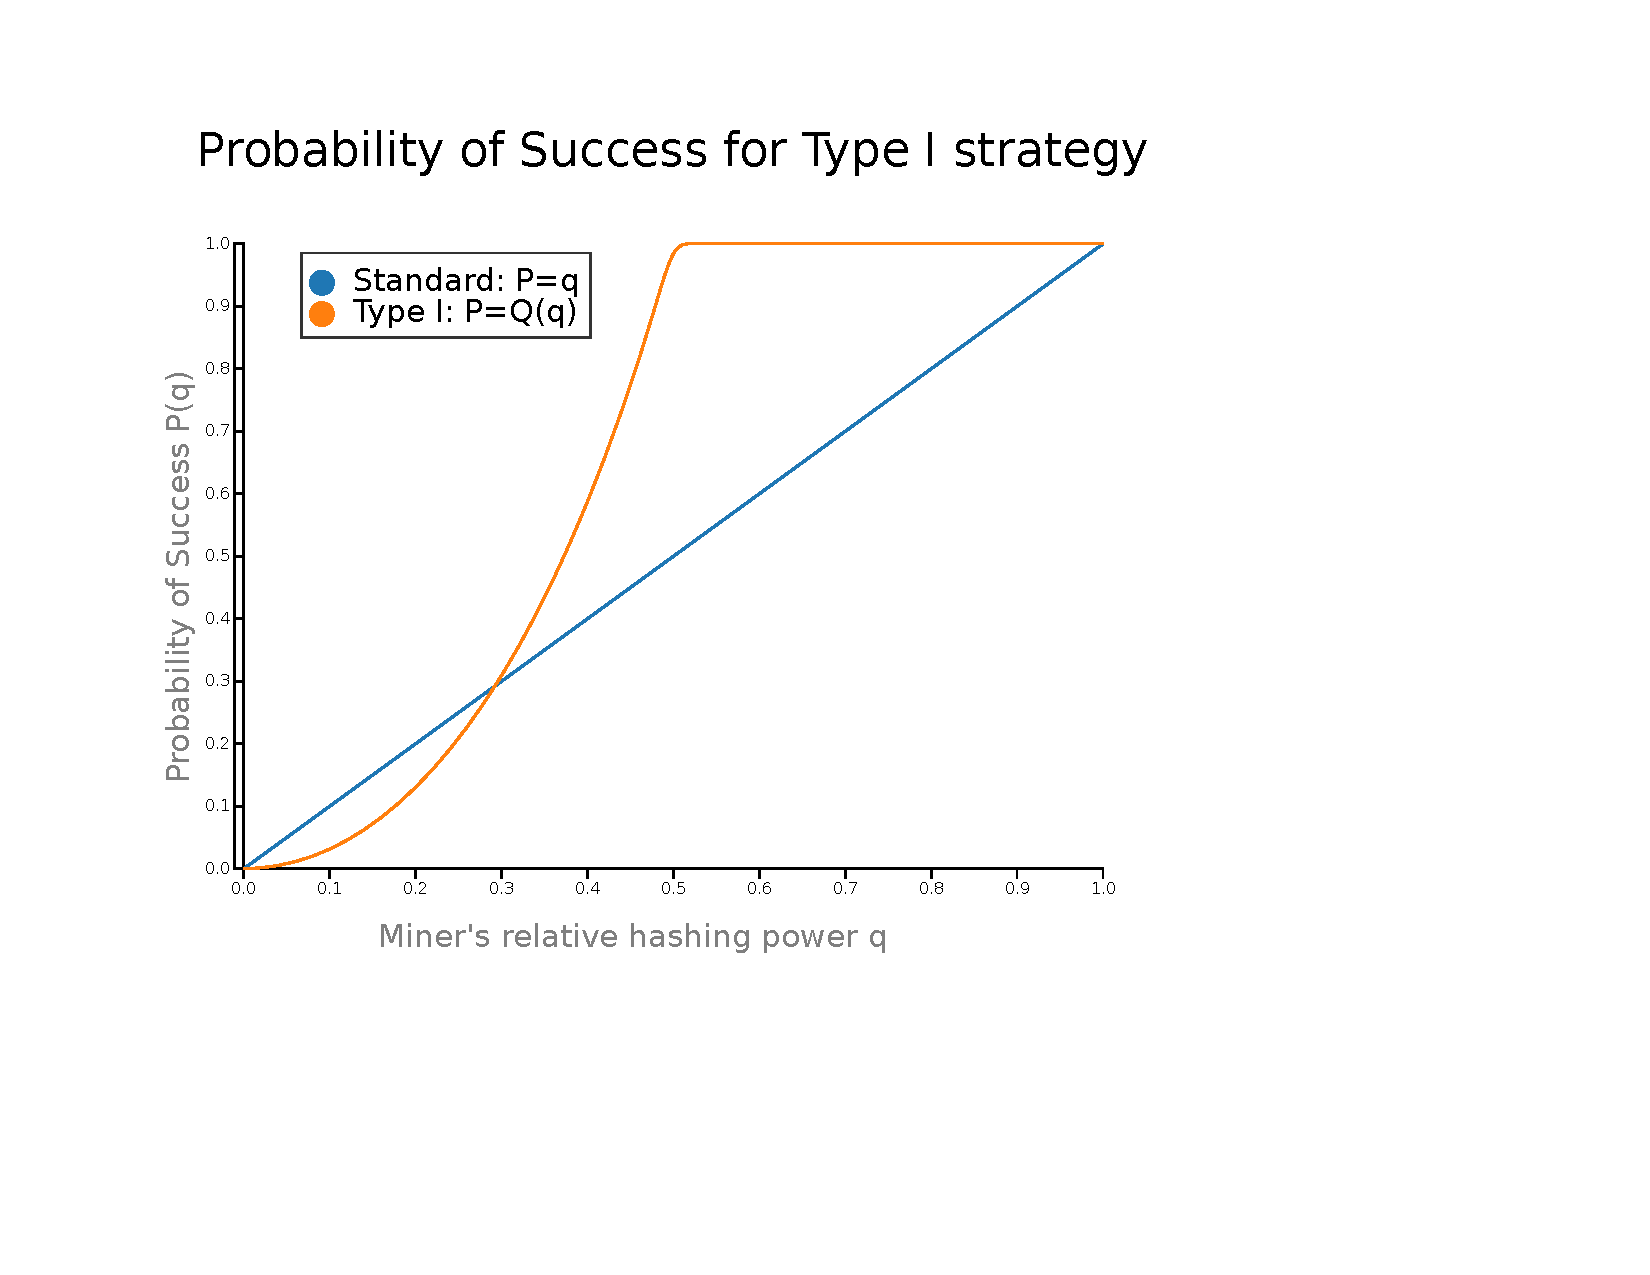
\includegraphics[keepaspectratio=true,scale=0.7]{TypeIPOS.pdf}}
\captionof{figure}{
The orange curve plots the probability that the attackers manage to uproot the next honest block and replace it with one of their own. The blue curve is the baseline probability for an honest miner with the same hashing power $q$
}
\label{fig:PlotProbOfSuccess}
\end{minipage}

\subsubsection{When is Type I better than Standard?}
To find out how big $q$ needs to be for this type of strategy to become more beneficial than the standard strategy we need to calculate:

\begin{equation}\label{eq:type1overstandard}
\dfrac{q^2}{1-q}\left(3-2q\right) \geq q
\end{equation}

which since $0\leq q \leq 1$ gives the condition $q \geq q_0$ where 

\begin{equation}\label{eq:qnot}
q_0=1-\frac{1}{\sqrt{2}} \sim 0.293
\end{equation}
We conclude that type I strategy is better than the standard strategy for $q>q_0$. Once $q\geq \frac{1}{2}$ we get to the famous ``$51\%$ attack" where the type I strategy is actually guaranteed to succeed.


\section{Block withholding attack - Type 0}
In this section we analyse the type 0 strategy probability of success.
Instead of publishing the secret branch when it is longer than the main branch, the miners that follow this strategy publish it one step before when the length of the secret branch is the same as the length of the main branch, i.e. when they reach a tie. The reason this is potentially beneficial is that due to latency effects in the bitcoin network (recently discussed in \cite{Zoharetal}) not all miners share the same view of the entire block-tree at all moments. All honest miners shift their efforts to the longest branch they know of, but for some short period of time different parts of the network may be aware of different, and equally valid, longest branches. In such a case, each sub-network continues mining it's branch until the next block is mined by either one of them and a new block-chain is established\footnote{In principle this type of block-chain bifurcation can continue to span multiple blocks, with exponentially decreasing probability.}. 
Following the notation used in \cite{Selfish} let us denote by $\gamma$ the ratio of standard miners that choose to mine on top of the Type 0 branch.
This means that $q+\gamma p$ of the total hashing power is now dedicated to making the attackers branch the longest. With some probability the attacker's branch ends up as the winner. Let us denote the probability that this type of tie strategy succeeds by $S_{\gamma}(q)$.
We can calculate $S_{\gamma}(q)$ starting the same way as we did when we derived \ref{eq:qofp} but use a Markov chain with boundary condition reflecting a tie instead of wining, and multiply that by the probability of an attacker with hashing power $q+\gamma p$ wining the race starting from that point.

Formally, we want to solve \ref{eq:markov} with boundary conditions $b_0=1, b_\infty=0$ which is solved by:

\begin{equation}\label{eq:bz}
\mathit{b}_z(q)=\begin{cases}\left( \dfrac{q}{1-q}\right)^z & q\in [0,\frac{1}{2}] \quad \mathrm{and} \quad z=0,1,2\dots \\ \quad 1 & \mathrm{otherwise} \end{cases}
\end{equation}

Using the same logic used to derive \ref{eq:qofpdef} we get the probability for a tie

\begin{equation}\label{eq:qofpdef}
\mathit{T}(q)= \sum_{m=0}^{\infty}\mathit{P}_{1,q}(m)\mathit{b}_{1-m}(q)
\end{equation}

resulting in (see details in appendix \ref{app:calctofp})

\begin{equation}\label{eq:qofp}
\mathit{T}(q)=
\begin{cases}
2q & \quad q \in [0,\frac{1}{2}] \\
1 & \quad q \in [\frac{1}{2},1] 
\end{cases}
\end{equation}

Now the attacker, joined by $\gamma$ of the honest miners are competing with the rest of the honest miners. The probability to win starting from a tie is thus given by \ref{eq:az}

\begin{equation}\label{eq:azeroeff}
\mathit{a}_0(q_{eff})=\begin{cases} \dfrac{q_{eff}}{1-q_{eff}} & q_{eff}\in [0,\frac{1}{2}] \\  
\quad 1 & q_{eff}\in [\frac{1}{2},1] \\ \end{cases}
\end{equation}

where 
\begin{equation}\label{qeff}
q_{eff}=q+\gamma p=q+\gamma(1-q)
\end{equation}

\begin{figure}[qcrit]
\centering
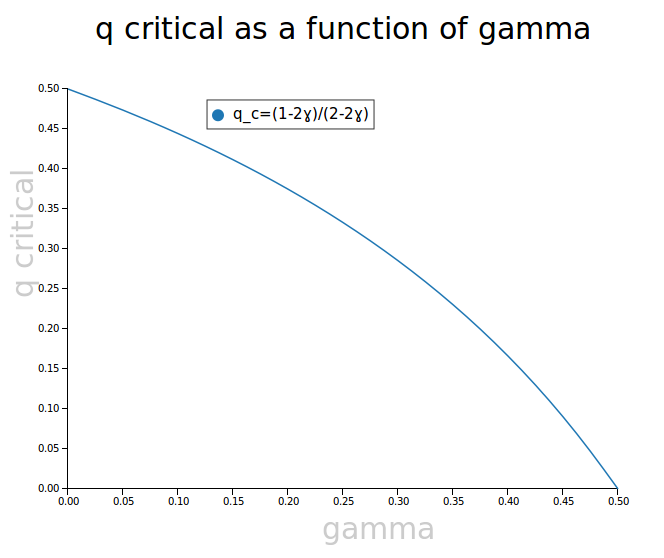
\includegraphics[width=100mm]{qcritical.png}
\caption{The value of $q_c$ as a function of $\gamma$.}
\label{fig:qcritical}
\end{figure}

The condition $q_{eff}\in [0,\frac{1}{2}]$ translates to $0\leq q\leq q_{c}(\gamma)$ where

\begin{equation}\label{qcrit}
q_{c}(\gamma)=\dfrac{1-2\gamma}{2-2\gamma}
\end{equation}

$q_c$ (depicted in figure \ref{fig:qcritical}) satisfies $0 \leq   q_{c}(\gamma) \leq\dfrac{1}{2}$, monotonically decreases with $\gamma$ and hits $0$ when\footnote{$q_{eff}(\frac{1}{2})=\frac{1}{2}(1+q)$ which is bigger than $\frac{1}{2}$ for any $q$.} $\gamma=\frac{1}{2}$.



Based on all that, the solution to $S_\gamma(q)=T(q)\cdot a_0(q_{eff})$ breaks into three regimes:

\begin{equation}\label{sofq}
S_\gamma(q)=\underbrace{T(q)}_{reach\; a\; tie}\cdot \underbrace{a_0(q_{eff})}_{win\;given\;a\;tie}=
\begin{cases}
2q\cdot\frac{q_{eff}}{1-q_{eff}}=2q\cdot\frac{q(1-\gamma)+\gamma}{(1-q)(1-\gamma)} & q\in [0,q_c] \\ 
2q & q\in [q_c,\frac{1}{2}] \\ 
1 & q\in [\frac{1}{2},1] \\ 
\end{cases}
\end{equation}

Note that if $\gamma\geq\frac{1}{2}$ the first regime does not exist and the solution degenerates to:

\begin{equation}\label{sofq2}
S_{\gamma\geq\frac{1}{2}}(q)=T(q)\cdot a_0(q_{eff})=
\begin{cases}
2q & q\in [0,\frac{1}{2}] \\ 
1 & q\in [\frac{1}{2},1] \\ 
\end{cases} \quad = min(2q,1)
\end{equation}

In figure \ref{fig:type0pos} we plot the probability of a successful type 0 attack for various values of the parameter $\gamma$, against the benchmark honest probability of success and the Type I attack probability of success.


\begin{figure}[blockwithholdingtype2]
\centering
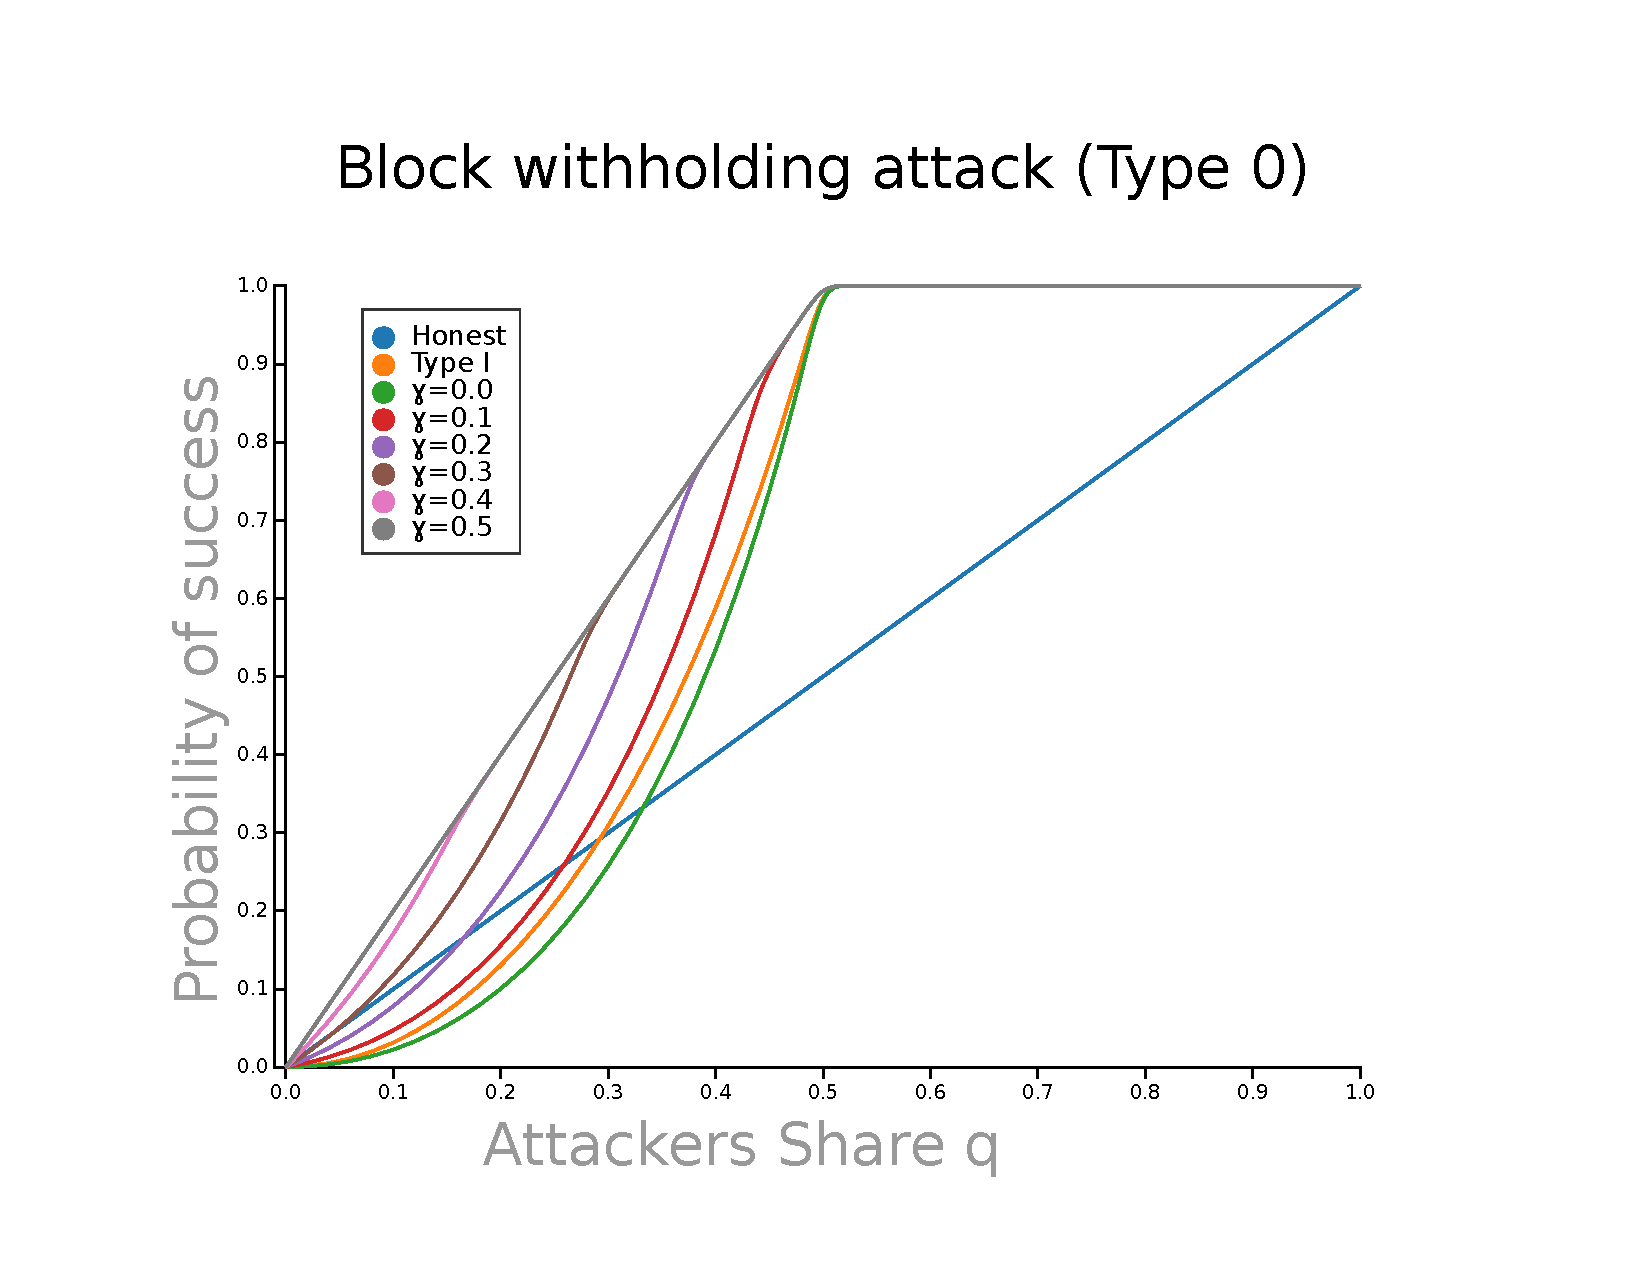
\includegraphics[width=200mm]{type0pos.pdf}
\caption{The probability of success of a type II block withholding attack as a function of $\gamma$. The blue curve plots the honest probability of success, and the orange curve plots the type I attack.}
\label{fig:type0pos}
\end{figure}

\section{The $\gamma,q$ phase space}\label{gqphase}

\subsection{When is a Type 0 attack beneficial}

To decide if a block-withholding attack of type 0 is beneficial or not we should compare it to the honest probability of success and to a Type I attack. 

\subsubsection{Comparing type 0 to the standard strategy}
First note that in the second and third regimes in equation \ref{sofq} (or for any $q$ if $\gamma\geq\frac{1}{2}$) the type 0 attacks is beneficial over the honest strategy for any $q$, because for any $q$ it holds that $0\leq q \leq min(2q,1)$. 

In the first regime (i.e. when $q<q_c(\gamma)$) we can find at what value of $q$ the type 0 attacks starts being beneficial over the honest strategy by solving
\begin{equation}\label{eq:type0benefitonhonestequation}
2q\cdot\frac{q(1-\gamma)+\gamma}{(1-q)(1-\gamma)}\geq q
\end{equation}

which gives the condition $q_b(\gamma)\leq q \leq q_c(\gamma)$, where 

\begin{equation}\label{eq:qb}
q_b= \dfrac{1-3\gamma}{3-3\gamma}
\end{equation}

The curve $q_b)\gamma)$ designating the boundary where the Type 0 strategy starts becoming more beneficial than the standard strategy is plotted in Figure \ref{fig:qbenefit}.

\begin{figure}[qcrit]
\centering
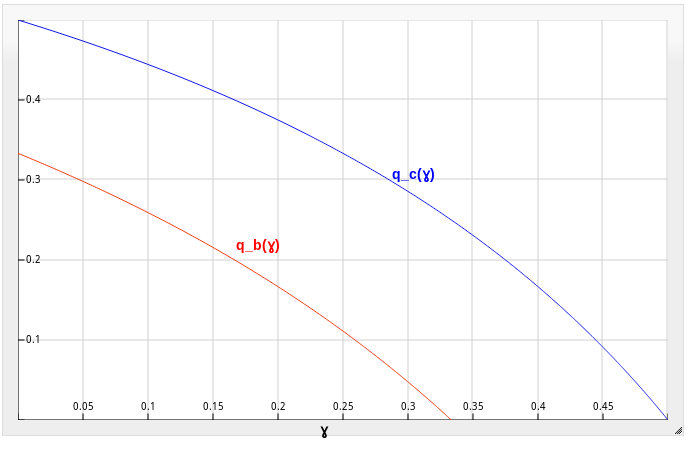
\includegraphics[width=100mm]{qcqb.png}
\caption{The value of $q_c$ and $q_b$ as a function of $\gamma$.}
\label{fig:qbenefit}
\end{figure}

Note that if $\gamma=0$ this strategy is beneficial only when $q>\frac{1}{3}$ and if $\gamma\geq\frac{1}{3}$ it is beneficial for all $q$.

\newpage

Taking all three regimes into account we conclude that the type 0 attack is beneficial over the honest strategy when

\begin{equation}\label{eq:0overhonest}
S_{\gamma}(q)\geq q \Longrightarrow
\begin{cases}
q>\dfrac{1-3\gamma}{3-3\gamma} & \gamma\in [0,\frac{1}{3}] \\ 
\mathit{any\;} q & \gamma\in [\frac{1}{3},1] \\ 
\end{cases}
\end{equation}

we can summarize further by writing

\begin{equation}\label{eq:0overhonestsummary}
S_{\gamma}(q)\geq q \Longrightarrow
q>max\left\lbrace\dfrac{1-3\gamma}{3-3\gamma},0\right\rbrace
\end{equation}

Next we compare this attack to a Type I attack.

\subsection{Comparing Type 0 to Type I}

There are two interesting comparisons one can make between Type 0 and Type I attacks.

One is to compare how they match against the honest strategy. Namely, for a given $\gamma$ do we first hit the regime where a Type 0 or a Type I strategy is more beneficial than the standard strategy.

This type 0 strategy wins earlier (in fact already at $q=0$) when $\gamma\geq\frac{1}{3}$. When $\gamma < \frac{1}{3}$ we can compare $q_b(\gamma)$ (given in equation \ref{eq:qb}) with $q_0$ (given in equation \ref{eq:qnot}).

\begin{equation}\label{eq:qbornot}
\dfrac{1-3\gamma}{3-3\gamma}<1-\dfrac{1}{\sqrt{2}}
\end{equation}

Solving for $\gamma$ we obtain that for  $\gamma_c\leq\gamma$ a type 0 strategy is beneficial over the standard strategy sooner (i.e. smaller $q$) than a type I strategy, where $\gamma_c$ is given by:

\begin{equation}\label{gamma0before1}
\gamma_c=1-\frac{2}{3}\sqrt{2}\sim 0.0572
\end{equation}

Indeed, you can see in Figure \ref{fig:type0pos} that the green curve representing $\gamma=0$ lies below the orange curve which represents the Type I strategy, while the red curve representing $\gamma=0.1>\gamma_c$ lies above it.

To summarize, when $\gamma\geq\frac{1}{3}$ the Type 0 strategy is beneficial over the honest strategy for any value of $q$. When $\gamma<\frac{1}{3}$ , the hashing power of the attacker needs to exceed a threshold before a block withholding strategy is beneficial. If $\gamma_c\leq\gamma\leq\frac{1}{3}$ we bump into the Type 0 first (the threshold given by $q_b=\frac{1-3\gamma}{3-3\gamma}$), while if $\gamma<\gamma_c$ we bump into Type I first (the threshold is given by $q_0=1-\frac{1}{\sqrt{2}}$).

Finally, ignoring the honest strategy for a moment, we can ask for the range of parameters $q,\gamma$ where the Type 0 strategy is more beneficial than the Type I strategy. Formally we need to solve:

\begin{equation}\label{eq:type0overtype1}
2q\cdot\frac{q(1-\gamma)+\gamma}{(1-q)(1-\gamma)}\geq \dfrac{q^2}{1-q}\left(
3-2q
\right)`
\end{equation}

which gives the condition

\begin{equation}\label{eq:type0over1condition}
2q^2-q+\frac{2\gamma}{1-\gamma}\geq 0
\end{equation}

This condition is satisfied in two regimes for $\gamma$.
\begin{equation}\label{eq:type0over1gammaregimes}
S_{\gamma}(q)\geq Q(q) \Longrightarrow
\begin{cases}
\mathit{any\;} q & \gamma\in [\frac{1}{17},1] \\ 
q<q_-(\gamma)\quad \mathit{or}\quad q>q_+(\gamma) & \gamma\in [0,\frac{1}{17}] \\ 
\end{cases}
\end{equation}

where 

\begin{equation}\label{qplusminus}
q_{\pm}(\gamma)=\frac{1}{4}\left(1\pm\sqrt{\frac{1-17\gamma}{1-\gamma}}\right)
\end{equation}


\section{The Strategy Phase Space}\label{sec:phasespace}

Now we can chart the strategy phase space parametrized by $\gamma,q$. 

Let us explore the $\gamma\in[0,1] \times q\in [0,1]$ phase space and divide it into regions characterized by the most beneficial mining strategy: \textbf{Standard}, \textbf{Type 0} or \textbf{Type I}.

The $\gamma, q$ phase space is governed by four functions (really three intersecting curves):
\begin{itemize}
\item $q_0= 1-\frac{1}{\sqrt{2}}$ determining for what $q$ type I is better than standard.
\item $max\lbrace q_b(\gamma)=\frac{1-3\gamma}{3-3\gamma},0\rbrace$ determining for what $q$ Type 0 is better than standard.
\item $q_+(\gamma)=\frac{1}{4}\left(1+\sqrt{\frac{1-17\gamma}{1-\gamma}}\right)$ 
\item $q_-(\gamma)=\frac{1}{4}\left(1-\sqrt{\frac{1-17\gamma}{1-\gamma}}\right)$
\end{itemize}
where the last two determine which strategy is better, Type 0 or I when $\gamma<\frac{1}{17}$.

\begin{figure}[fourfunctions]
\centering
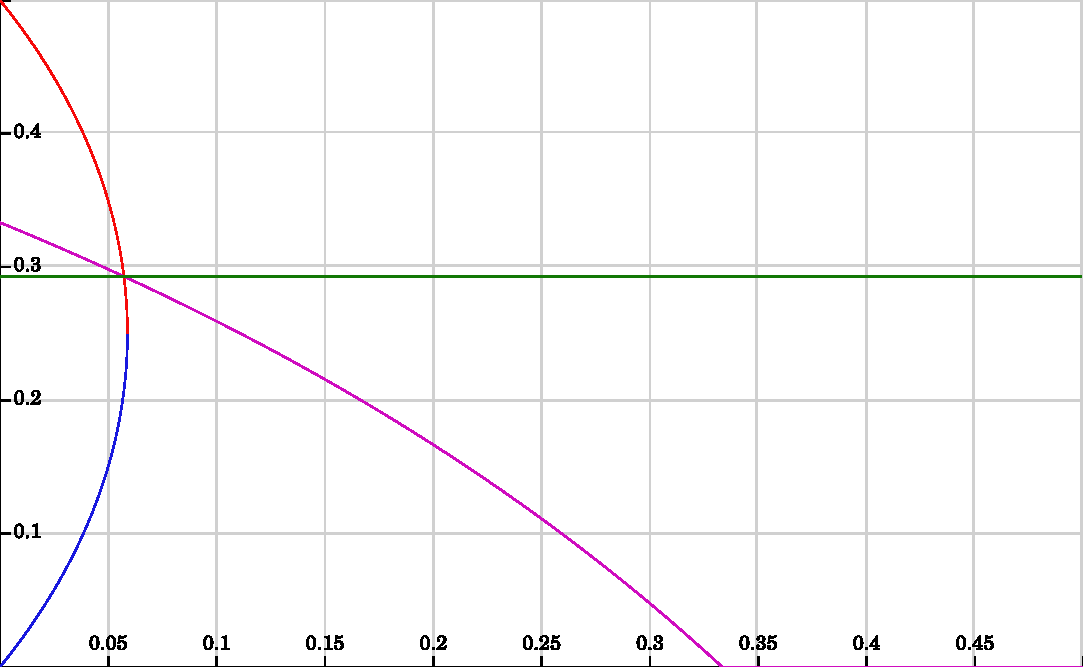
\includegraphics[width=150mm]{intersection4.pdf}
\caption{The 4 functions sectioning the $\gamma, q$ phase space.}
\label{fig:fourfunctions}
\end{figure}

In figure \ref{fig:fourfunctions} we those three curves are plotted.
Note the interesting fact that all three curves intersect in the single point $\gamma=\gamma_c, q=q_0$.
This fact makes the phase space much simpler to analyse.

\newpage

\begin{itemize}
\item The circular curve created by the two branches $q_{\pm}$ determines, for a given $\gamma$, which of the two block-withholding strategies, Type 0 or Type I is more beneficial. Inside the circular region (and all the way to the $q$ axis) is the region where Type I is better than type 0. Outside this region Type 0 is better than Type 1. This is determined by equation \ref{eq:type0over1condition}. Note that this division doesn't specify whether any of the strategies is better than the standard one.
\item The Type I strategy is more beneficial than the standard strategy in the region above the horizontal line $q=q_0$. .
\item The Type 0 strategy is more beneficial than the Standard strategy in the region above the monotonically decreasing curve $q_b(\gamma)$ (extending from $\frac{1}{3}$ on the $q$ axis to $\frac{1}{3}$ on the $\gamma$ axis and the continuing on the $\gamma$ axis all the way to $\gamma=1$).
\end{itemize}

The resulting phase space division is thus given by figure \ref{fig:qgammaphasespace}.

\begin{figure}[qgammaphasespace]
\centering
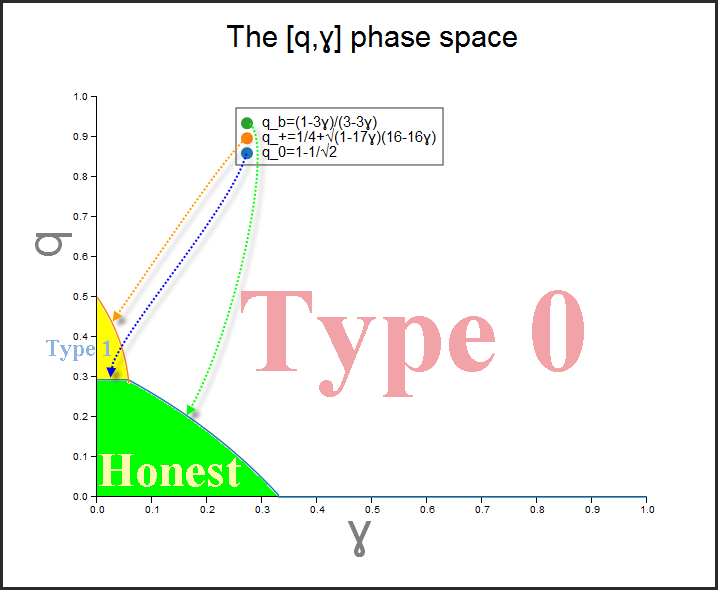
\includegraphics[width=130mm]{simpleqgammaphasespace.png}
\caption{The 3 regions of the $q,\gamma$ phase space. The standard strategy is best in the region near the origin. Type I is best in the little area on top of the standard region. In the rest of phase space the Type 0 strategy is most beneficial.}
\label{fig:qgammaphasespace}
\end{figure}


\newpage

Note that the regime where either block-withholding strategies are more beneficial than the standard strategy is bounded away from the origin. It is tempting to look at the radial distance from the origin of phase space as a measure of a ``miner's \textit{strength}" $\mathtt{S}(q,\gamma)\equiv \sqrt{q^2+\gamma^2}$.

This definition is partly motivated by the intuitive notion that having a large $\gamma$ is (in some vague sense) ``similarly difficult" to having a large $q$ and a typical miner will have both parameters in similar scales. In a sense, the above phase space diagram lends credibility to this intuitive notion because it suggest a rough symmetry\footnote{All we mean by that is that figure \ref{fig:qgammaphasespace} is almost symmetric under a rotation along the $45^\deg$ angle that rotates $\gamma \leftrightarrow q$.} between the parameters $\gamma$ and $q$.

There are a few remarks in order:
\begin{itemize}
\item Figure \ref{fig:qgammaphasespace} marks the regions where a block-withholding strategy in beneficial, but does not guarantee success. Success of either strategies is still guaranteed (i.e. the probability of success is strictly $1$) only in the top half of phase space, in the region where $q\geq \frac{1}{2}$, a.k.a the $51\%$ attack.
\item The authors of \cite{Selfish} identified a region delimited by the curve $\frac{1-\gamma}{3-2\gamma}\leq q \leq \frac{1}{3}$ where the ``selfish" mining strategy is more beneficial than the standard one. As one would expect based on the fact that the ``selfish'' strategy utilizes a combination of the two strategies discussed here, this curve intersects both Type I and Type 0 regions as depicted in \ref{fig:selfish}.
\end{itemize}



\appendix
\chapter{Calculation Details}
\section{Probability distribution} \label{app:probmath}

To find the normalization in the case $n>0$ we use the useful binomial identity holding for any complex $s$ inside the unit circle ($|s|<1$)

\dfrac{1}{(1-s)^n}=\sum_{k=0}^{\infty} {n + k -1\choose k}s^k.

It is now straightforward to show that \ref{eq:pnm} is indeed a probability distribution

\sum_{m=0}^{\infty}\mathit{P}(n,m,p)=p^n\sum_{m=0}^{\infty}{n + m -1\choose m}q^m=p^n\dfrac{1}{(1-q)^n}=1

\section{Calculating $\mathit{Q}(q)$ } \label{app:calcqofp} 

$\mathit{Q}(q)$  can be solved in the two regions for the parameter $q$ given in \ref{eq:az}.

In the case  that $q\in [0,\frac{1}{2}]$

\begin{eqnarray}\label{eq:rpcalc}\nonumber
&\mathit{Q}(q)=\sum_{m=0}^{\infty}\mathit{P}_{1,q}(m)\mathit{a}_{1-m}(q)=p\sum_{m=0}^{\infty}q^m\mathit{a}_{1-m}(p)=p\left(
\mathit{a}_1(p)+q\mathit{a}_0(p)+\sum_{m=2}^{\infty}q^m
 \right)=\\\nonumber
 &p\left(
\left(\dfrac{q}{p}\right)^2+q\dfrac{q}{p}+\left(\sum_{m=0}^{\infty}q^m\right)-1-q
 \right) 
 =p\left(
\left(\dfrac{q}{p}\right)^2+\dfrac{q^2p}{p^2}+\dfrac{1}{p}-(1+q)
 \right)=\\\nonumber
&\dfrac{1}{p}\left(
q^2(1+p)+p-p^2(1+q)
\right) 
 =\dfrac{1}{p}
\left(q^2(1+p)+p-p^2(1+q)
 \right)=\\\nonumber
&\dfrac{1}{1-q}\left(
q^2(2-q)+1-q-(1-q)^2(1+q)
\right) 
 =\\\nonumber
 &\dfrac{1}{1-q}\left(
2q^2-q^3+1-q-1+2q-q^2 -q+2q^2-q^3
\right) = \dfrac{q^2}{1-q}\left(
3-2q
\right)
\end{eqnarray}

In the case  that $q\in [\frac{1}{2},1]$

\begin{eqnarray}\nonumber
&\mathit{Q}(q)=p\sum_{m=0}^{\infty}q^m\mathit{a}_{1-m}(p)=p\left(
\mathit{a}_1(p)+q\mathit{a}_0(p)+\sum_{m=2}^{\infty}q^m
 \right)=\\\nonumber
 &p
\left(1+q+\left(\sum_{m=0}^{\infty}q^m\right)-1-q
 \right) 
 =p\dfrac{1}{p}=1
\end{eqnarray}

\section{Calculating $\mathit{T}(q)$ } \label{app:calctofp} 

$\mathit{T}(q)$  can be solved in the two regions for the parameter $q$ given in \ref{eq:az}.

In the case  that $q\in [0,\frac{1}{2}]$

\begin{eqnarray}\label{eq:rpcalc}\nonumber
&\mathit{Q}(q)=\sum_{m=0}^{\infty}\mathit{P}_{1,q}(m)\mathit{b}_{1-m}(q)=p\sum_{m=0}^{\infty}q^m\mathit{b}_{1-m}(p)=p\left(
\mathit{b}_1(q)+\sum_{m=1}^{\infty}q^m
 \right)=\\\nonumber
 &p\left(
\dfrac{q}{p}+\left(\sum_{m=0}^{\infty}q^m\right)-1
 \right) 
 =p\left(
\dfrac{q}{p}+\dfrac{1}{1-q}-1
 \right)=q+1-p=2q.\\\nonumber
\end{eqnarray}

The case $q\in [\frac{1}{2},1]$ is identical to the one carried above for $\mathit{Q}(q)$.


\begin{comment}
--------------------------------
\section{Calculating $\mathit{R}(p)$ } \label{app:calcrofp}  

$\mathit{R}(p)$  can be solved in the two regions for the parameter $q$ given in \ref{eq:az}.

In the case  that $q\in [0,\dfrac{1}{2}]$

\begin{eqnarray}\label{eq:rpcalc}\nonumber
&\mathit{R}(p)=p\sum_{m=0}^{\infty}m\cdot q^m\mathit{a}_{1-m}(p)=p\left(
q\mathit{a}_0(p)+\sum_{m=2}^{\infty}m\cdot q^m
 \right)=\\\nonumber
 &p\left(
q\dfrac{q}{p}+\left(\sum_{m=0}^{\infty}m\cdot q^m\right)-q
 \right) 
 =p\left(
\dfrac{q^2}{p}+q\partial_q\left(\sum_{m=0}^{\infty} q^m\right)-q
 \right)=\\\nonumber
& q^2+pq\partial_q\left(\dfrac{1}{1-q}\right)-pq 
 = q^2+pq\left(\dfrac{1}{p^2} -1\right) =q^2+q\dfrac{(1+p)(1-p)}{p}=
 \\\nonumber
& q^2\left(1+\dfrac{2-q}{1-q}\right)= \dfrac{q^2}{1-q}\left(
3-2q\right)=\mathit{Q}(p)
\end{eqnarray}


In the case  that $q\notin [0,\dfrac{1}{2}]$

\begin{eqnarray}\nonumber
&\mathit{R}(p)=p\sum_{m=0}^{\infty}m\cdot q^m\mathit{a}_{1-m}(p)=p\left(
q\mathit{a}_0(p)+\sum_{m=2}^{\infty}m\cdot q^m
 \right)=\\\nonumber
 & p\left(q+\left(\sum_{m=0}^{\infty}m\cdot q^m\right)-q \right) =pq\partial_q\left(\dfrac{1}{1-q}\right)=\dfrac{q}{1-q}
\end{eqnarray}

------------------------------
We start by noting some simple facts.
\begin{itemize}
\item Equation \ref{eq:qnot} tells us that in the regime $q>q_0=1-\frac{1}{\sqrt{2}}$ the Type I strategy is more beneficial than the standard strategy.
\item Equation \ref{eq:0overhonest} tells us that in the regime $\gamma\geq\frac{1}{3}$ The Type 0 strategy is more beneficial than the standard strategy.
\item Equation \ref{eq:type0over1gammaregimes} tells us that when $\frac{1}{17}\leq \gamma \leq \frac{1}{3}$ Type 0 is more beneficial than Type I for any $q$, so we only need to ask when is Type 0 better than the standard strategy, and we get the answer from equations \ref{eq:type0benefitonhonestequation} and \ref{eq:qb} to be $q>q_b(\gamma)=\frac{1-3\gamma}{3-3\gamma}$.
\end{itemize}

The rest of phase space requires some more analysis.

\subsubsection{The regime $\gamma_c=1-\frac{2\sqrt{2}}{3}\sim 0.0572\leq \gamma \leq \frac{1}{17}\sim 0.0588$ }

By definition of $\gamma_c$ (equation \ref{eq:qbornot}) in this region $q_b(\gamma)<q_0$.
Thus, this region in $\gamma$ breaks up into three regions in $q$. Namely:

\begin{itemize}
\item $q\leq q_b(\gamma)$ In this region neither block withholding strategies are better than the standard strategy, and so a miner will follow the standard strategy.
\item $q_b(\gamma)\leq q\leq q_0$ In this region Type 0 is better than the standard strategy and type I is not and so a miner will choose the Type 0 strategy.
\item $q_0\leq q$ In this region both Type 0 and type I are better than the standard strategy and so we need to measure them up against each other to find out which one wins.

\end{itemize}

In this region we learn from equation \ref{eq:type0over1gammaregimes} that Type 0 is better than Type I only if $q<q_-(\gamma)$ or $q>q_+(\gamma)$. 
Let us first attempt to solve for $q_b(\gamma)\leq q < q_-(\gamma)$. For this to be possible we must have $q_b(\gamma)\leq q_-(\gamma)$, or:

\begin{equation}
\frac{1}{4}\left(1-\sqrt{\frac{1-17\gamma}{1-\gamma}}\right)\geq 1-\frac{1}{\sqrt{2}}
\end{equation}

which gives 

\begin{equation}
\frac{1}{4}\sqrt{\frac{1-17\gamma}{1-\gamma}}\leq \frac{1}{\sqrt{2}}-\frac{3}{4}<0
\end{equation}

having no solutions.

However, there is still the option that Type I wins in this region if we can find a solution where $q_0<q\leq q_+(\gamma)$.
For this to be possible we need $q_+(\gamma)>q_0$:
\begin{equation}
\frac{1}{4}\left(1+\sqrt{\frac{1-17\gamma}{1-\gamma}}\right)\geq 1-\frac{1}{\sqrt{2}}
\end{equation}
which gives 

\begin{equation}
\frac{1}{4}\sqrt{\frac{1-17\gamma}{1-\gamma}}\leq \frac{3}{4}-\frac{1}{\sqrt{2}}>0
\end{equation}

In this case a solution exists, giving the condition $\gamma<\gamma_c$:
Since we are analysing the region $\gamma_c\leq \gamma$ we see that in this region the type I strategy is never more beneficial than the Type 0 strategy and thus we conclude that in the region $\gamma_c\leq \gamma \leq \frac{1}{17}$ 
\begin{itemize}
\item $q\leq q_b(\gamma)$ - Standard strategy wins
\item $q_b(\gamma)\leq q$ - Type 0 strategy wins
\end{itemize}

Finally, 




All this results in the following division of phase space:

\begin{figure}[sectioning]
\centering
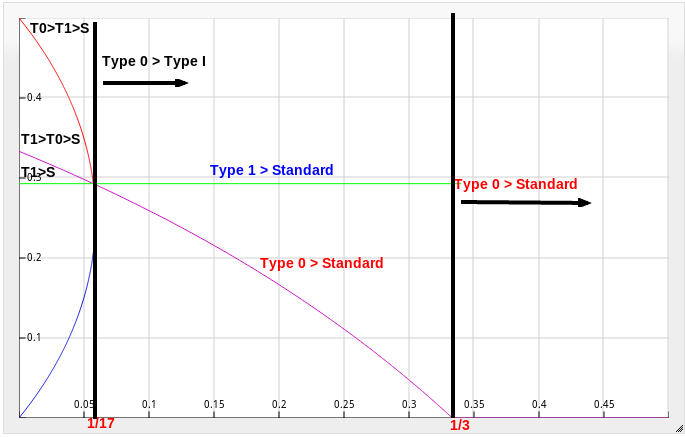
\includegraphics[width=150mm]{sectioning.png}
\caption{The 4 functions sectioning the $\gamma, q$ phase space.}
\label{fig:sectioning}
\end{figure}

Leading to figure \ref{fig:qgammaphasespace}.
---------------------------------------------------
\end{comment}



\newpage
\bibliographystyle{plain} % IEEEtr, plain, abbrv, alpha
\addcontentsline{toc}{chapter}{Bibliography}
\bibliography{blocksurvival}
\end{document} %\input{bibliography}
